
\de{ĐỀ THI HỌC KỲ I NĂM HỌC 2022-2023}{THPT Chuyên Lương Văn Tụy - Ninh Bình}
\begin{center}
	\textbf{PHẦN 1 - TRẮC NGHIỆM}
\end{center}
\Opensolutionfile{ans}[ans/ans]
%Câu 1...........................
\begin{ex}%[0H3Y1-3]%[Dự án đề kiểm tra HKI NH22-23- Phạm Phương]%[THPT Lương Văn Tụy - Sở Ninh Bình]
	Trong mặt phẳng toạ độ $Oxy$, cho hai điểm $A(1;4)$ và $B(3;5)$. Khi đó
	\choice
	{$\overrightarrow{AB}=(-2;-1)$}
	{$\overrightarrow{AB}=(4;9)$}
	{$\overrightarrow{AB}=(1;2)$}
	{\True $\overrightarrow{AB}=(2;1)$}
	\loigiai{
	$$\overrightarrow{AB}=\left(3-1;5-4\right)=(2;1).$$
	}
\end{ex}
\begin{ex}%[0H3Y1-3]%[Dự án đề kiểm tra HKI NH22-23- Phạm Phương]%[THPT Lương Văn Tụy - Sở Ninh Bình]
	Trong mặt phẳng tọa độ $Oxy$, cho $A(-2;0)$, $B(5;-4)$. Tọa độ trung điểm $I$ của $AB$ là
	\choice
	{$I(3;-4)$}
	{\True $I\left(\dfrac{3}{2};-2\right)$}
	{$I\left(\dfrac{2}{3};-2\right)$}
	{$I\left(\dfrac{3}{2};2\right)$}
	\loigiai{
	Gọi $I\left(x_I;y_I\right)$ là trung điểm của $AB$ ta có 
	$$\heva{&x_I=\dfrac{(-2)+5}{2}=\dfrac{3}{2}\\& x_I=\dfrac{0+(-4)}{2}=-2} \Rightarrow I\left(\dfrac{3}{2};-2\right).$$
}
\end{ex}
\begin{ex}%[0D1Y2-3]%[Dự án đề kiểm tra HKI NH22-23- Phạm Phương]%[THPT Lương Văn Tụy - Sở Ninh Bình]
	Cho $A=[-2;7)$, $B=(3;+\infty)$. Khi đó $A \cup B$ bằng
	\choice
	{\True $[-2;+\infty)$}
	{$(3;7)$}
	{$[-2;3)$}
	{$(-2;+\infty)$}
	\loigiai{
	Ta có $A \cup B= [-2;7) \cup (3;+\infty) = \left[-2;+\infty\right)$.
}
\end{ex}
\begin{ex}%[0D3Y1-4]%[Dự án đề kiểm tra HKI NH22-23- Phạm Phương]%[THPT Lương Văn Tụy - Sở Ninh Bình]
	Điểm nào dưới đây thuộc đồ thị của hàm số $y=x^3-x+2$?
	\choice
	{\True Điểm $P(1;2)$}
	{Điểm $M(1;1)$}
	{Điểm $Q(1;3)$}
	{Điểm $N(1;0)$}
	\loigiai{
	Với $x=1$ ta có $y=1^3-1+2=2$ suy ra điểm $P(1;2)$ thuộc đồ thị của hàm số $y=x^3-x+2$.
}
\end{ex}
\begin{ex}%[0H1Y2-1]%[Dự án đề kiểm tra HKI NH22-23- Phạm Phương]%[THPT Lương Văn Tụy - Sở Ninh Bình]
	Trong tam giác $ABC$ mệnh đề nào đúng?
	\choice
	{$a^2=b^2+c^2-ac \cdot \cos A$}
	{$a^2=b^2+c^2+2bc \cdot \cos A$}
	{\True $a^2=b^2+c^2-2bc \cdot \cos A$}
	{$a^2=b^2+c^2+bc \cdot \cos A$}
	\loigiai{
	Theo định lý cô-sin ta có $a^2=b^2+c^2-2bc \cdot \cos A$.
}
\end{ex}
\begin{ex}%[0D2Y1-1]%[Dự án đề kiểm tra HKI NH22-23- Phạm Phương]%[THPT Lương Văn Tụy - Sở Ninh Bình]
	Bất phương trình nào sau đây là bất phương trình bậc nhất hai ẩn?
	\choice
	{$x-y^2>0$}
	{$3x^2+y^2 \leq 0$}
	{\True $5x-y \geq 0$}
	{$3x^2+2y<0$}
	\loigiai{
	Bất phương trình $5x-y \geq 0$ là bất phương trình bậc nhất hai ẩn.
}
\end{ex}
\begin{ex}%[0X1Y1-3]%[Dự án đề kiểm tra HKI NH22-23- Phạm Phương]%[THPT Lương Văn Tụy - Sở Ninh Bình]
	Sử dụng máy tính bỏ túi, hãy viết giá trị gần đúng của $\sqrt{3}$ chính xác đến hàng phần nghìn.
	\choice
	{$1{,}733$}
	{$1{,}731$}
	{\True $1{,}732$}
	{$1{,}73$}
	\loigiai{
	Ta có $\sqrt{3}\approx 1{,}732050808$ nên giá trị gần đúng của $\sqrt{3}$ chính xác đến hàng phần nghìn là $1{,}732$.
}
\end{ex}
\begin{ex}%[0H1B1-2]%[Dự án đề kiểm tra HKI NH22-23- Phạm Phương]%[THPT Lương Văn Tụy - Sở Ninh Bình]
	Cho $\cos \alpha=-\dfrac{2}{5}$, $\left(90^{\circ}<\alpha<180^{\circ}\right)$. Khi đó $\tan \alpha$ bằng
	\choice
	{\True $-\dfrac{\sqrt{21}}{2}$}
	{$\dfrac{\sqrt{21}}{2}$}
	{$-\dfrac{\sqrt{21}}{5}$}
	{$\dfrac{\sqrt{21}}{3}$}
	\loigiai{
	Ta có $1+tan^2\alpha=\dfrac{1}{\cos^2\alpha} \Rightarrow \tan^2\alpha=\dfrac{1}{\cos^2\alpha}-1=\dfrac{1}{\left(-\tfrac{2}{5}\right)^2}-1=\dfrac{21}{4}$.
	\\
	Vì  $90^{\circ}<\alpha<180^{\circ}$ nên $\tan\alpha<0$ suy ra $\tan\alpha=-\sqrt{\dfrac{21}{4}}=-\dfrac{\sqrt{21}}{2}$.
}
\end{ex}
\begin{ex}%[0H1B1-2]%[Dự án đề kiểm tra HKI NH22-23- Phạm Phương]%[THPT Lương Văn Tụy - Sở Ninh Bình]
	\immini{
	Biểu diễn miền nghiệm được cho bởi hình bên (phần không bị tô đậm kể cả đường thẳng) là miền nghiệm của bất phương trình nào?
	\choice
	{$2x+y-1>0$}
	{$2x+y-2=0$}
	{\True $2x+y-2 \leq 0$}
	{$2x+y+2 \leq 0$}
}{
\begin{tikzpicture}[scale=0.8,>=stealth, font=\footnotesize, line join=round, line cap=round]
	\def\xmin{-2} \def\xmax{2.5}
	\def\ymin{-1} \def\ymax{3.5}
	%\draw[color=gray!50,dashed] (\xmin,\ymin) grid (\xmax,\ymax);	
	\draw[->] (\xmin,0)--(\xmax,0) node [below]{$x$};
	\draw[->] (0,\ymin)--(0,\ymax) node [left]{$y$};
	\fill (0,0) circle (1pt) node[shift={(-135:3mm)}]{$O$};
	\clip (\xmin+0.1,\ymin+0.1) rectangle (\xmax-0.1,\ymax-0.1);
	\draw[smooth,samples=300] plot(\x,{-2*(\x)+2});
	\fill[pattern=north east lines,pattern color=blue,opacity=.7]plot[domain=\xmin:\xmax](\x,{-2*(\x)+2})--plot[domain=\xmax:\xmin](\x,{\ymax})--cycle;
	\fill (1,0) circle (1pt) node[shift={(-135:3mm)}]{$1$};
	\fill (0,2) circle (1pt) node[shift={(-170:3mm)}]{$2$};
\end{tikzpicture}
}
	\loigiai{
	Đường thẳng đi qua $(1;0)$ và $(0;2)$ nên thuộc đường thẳng $2x+y-2=0$.
	\\
	Lại có điểm $O(0;0)$ thuộc miền nghiệm nên miền nghiệm đã cho là miền nghiệm của bất phương trình $2x+y-2 \leq 0$.
}
\end{ex}
\begin{ex}%[0X1Y3-2]%[Dự án đề kiểm tra HKI NH22-23- Phạm Phương]%[THPT Lương Văn Tụy - Sở Ninh Bình]
	Một nhóm $10$ học sinh tham gia một kỳ thi. Số điểm thi của 10 học sinh đó được sắp xếp từ thấp đến cao như sau (thang điểm $10$): $0;\ 1;\ 2;\ 4;\ 4;\ 5;\ 7;\ 8;\ 8;\ 9$. Khi đó số trung vị của mẫu số liệu trên bằng
	\choice
	{$5{,}5$}
	{$4$}
	{\True $4{,}5$}
	{$5$}
	\loigiai{
	Mẫu có $10$ số liệu nên số trung vị là trung bình cộng của hai số ở vị trí thứ $5$ và $6$, do đó
	$$M_e=\dfrac{4+5}{2}=4{,}5.$$
}
\end{ex}
\begin{ex}%[0D2Y2-2]%[Dự án đề kiểm tra HKI NH22-23- Phạm Phương]%[THPT Lương Văn Tụy - Sở Ninh Bình]
	Điểm nào sau đây thuộc miền nghiệm của hệ bất phương trình $\heva{&3x-4y+12 \geq 0 \\& x+y-2>0}$
	\choice
	{$M(0;4)$}
	{$N(2;0)$}
	{$Q(1;1)$}
	{\True $P(0;3)$}
	\loigiai{
	Xét điểm $P(0;3)$ có $\heva{&3\cdot 0 -4\cdot 3+12 \geq 0 \\& 0+3-2>0} \Leftrightarrow \heva{&0 \geq 0 \,\text{(đúng)}\\& 1>0 \,\text{(đúng)}.}$
	\\
	Do đó $P(0;3)$ thuộc miền nghiệm của hệ bất phương trình đã cho.
}
\end{ex}
\begin{ex}%[0D3Y1-2]%[Dự án đề kiểm tra HKI NH22-23- Phạm Phương]%[THPT Lương Văn Tụy - Sở Ninh Bình]
	Tập xác định của hàm số $y=\dfrac{1}{x-6}$ là
	\choice
	{\True $\mathbb{R} \setminus \{6\}$}
	{$(6;+\infty)$}
	{$[6;+\infty)$}
	{$(-\infty;6)$}
	\loigiai{
	Hàm số $y=\dfrac{1}{x-6}$ có nghĩa khi $x-6 \neq 0 \Leftrightarrow x \neq 6$.
	\\
	Vậy tập xác định của hàm số $y=\dfrac{1}{x-6}$ là $\mathscr{D}=\mathbb{R} \setminus \{6\}$.
}
\end{ex}
\begin{ex}%[0H2B3-1]%[Dự án đề kiểm tra HKI NH22-23- Phạm Phương]%[THPT Lương Văn Tụy - Sở Ninh Bình]
	Trên đoạn thẳng $AB$ lấy điểm $I$ sao cho $AB=4AI$. Chọn khẳng định đúng.
	\vspace{-0.4cm}
	\begin{center}
		\begin{tikzpicture}[scale=0.8,>=stealth, font=\footnotesize, line join=round, line cap=round]
			\foreach \i/\j/\k in{0/0/A,1/0/I,4/0/B,2/0/M,3/0/N}
			\coordinate (\k) at(\i,\j);
			\draw (A)--(B);
			\foreach \p/\r in {A/135,B/45,I/90}
			\fill (\p) circle (1pt) node[shift={(\r:3mm)}]{$\p$};
			\fill (M) circle (1pt);	
			\fill (N) circle (1pt);
		\end{tikzpicture}
	\end{center}
	\choice
	{$\overrightarrow{IB}=\dfrac{-3}{4} \overrightarrow{AB}$}
	{$\overrightarrow{IB}=\dfrac{4}{3} \overrightarrow{AB}$}
	{$\overrightarrow{IB}=3 \overrightarrow{IA}$}
	{\True $\overrightarrow{IB}=-3 \overrightarrow{IA}$}
	\loigiai{
	Ta có $IB=3IA$ và $\overrightarrow{IB}$, $\overrightarrow{IA}$ ngược hướng nên $\overrightarrow{IB}=-3 \overrightarrow{IA}$.
}
\end{ex}
\begin{ex}%[0H1Y1-2]%[Dự án đề kiểm tra HKI NH22-23- Phạm Phương]%[THPT Lương Văn Tụy - Sở Ninh Bình]
	Trong các đẳng thức sau đây, đẳng thức nào đúng?
	\choice
	{\True $\tan 150^{\circ}=-\dfrac{\sqrt{3}}{3}$}
	{$\cos 150^{\circ}=\dfrac{\sqrt{3}}{2}$}
	{$\sin 150^{\circ}=-\dfrac{\sqrt{3}}{2}$}
	{$\cot 150^{\circ}=\sqrt{3}$}
	\loigiai{
	Ta có $\tan 150^{\circ}=-\tan 30^{\circ} =-\dfrac{\sqrt{3}}{3}$.
}
\end{ex}
\begin{ex}%[0D1Y3-4]%[Dự án đề kiểm tra HKI NH22-23- Phạm Phương]%[THPT Lương Văn Tụy - Sở Ninh Bình]
	Cho tập hợp $C=\{x \in \mathbb{R} \mid -4 \leq x \leq 0\}$. Tập hợp $C$ được viết dưới dạng tập hợp nào sau đây?
	\choice
	{$C=(-4;0]$}
	{$C=(-4;0)$}
	{$C=[-4;0)$}
	{\True $C=[-4;0]$}
	\loigiai{
	$C=\{x \in \mathbb{R} \mid -4 \leq x \leq 0\} \Leftrightarrow C=[-4;0]$.
}
\end{ex}
\begin{ex}%[0H1B2-1]%[Dự án đề kiểm tra HKI NH22-23- Phạm Phương]%[THPT Lương Văn Tụy - Sở Ninh Bình]
	Cho tam giác $ABC$ biết $a=24$, $b=13$, $c=15$. Tính góc $A$.
	\choice
	{$A=33^{\circ} 34'$}
	{$A=28^{\circ} 37'$}
	{\True $A=117^{\circ} 49'$}
	{$A=58^{\circ} 24'$}
	\loigiai{
	Theo hệ quả định lý cô-sin ta có
	\allowdisplaybreaks{
		\begin{eqnarray*}
			& & \cos A=\dfrac{b^2+c^2-a^2}{2bc}=\dfrac{13^2+15^2-24^2}{2\cdot 13\cdot 15}=-\dfrac{7}{15}\\
			&\Rightarrow & \widehat{A}\approx 117^{\circ} 49'.
	\end{eqnarray*} }
}
\end{ex}
\begin{ex}%[0D3Y2-3]%[Dự án đề kiểm tra HKI NH22-23- Phạm Phương]%[THPT Lương Văn Tụy - Sở Ninh Bình]
	Đỉnh của parabol $y=3x^2+2x-5$ có hoành độ bằng
	\choice
	{$-\dfrac{2}{3}$}
	{$\dfrac{1}{3}$}
	{$\dfrac{2}{3}$}
	{\True $-\dfrac{1}{3}$}
	\loigiai{
	Hoành độ đỉnh $S$ của parabol là $x_S=-\dfrac{b}{2a}=-\dfrac{2}{2\cdot 3}=-\dfrac{1}{3}$.
}
\end{ex}
\begin{ex}%[0D3B2-4]%[Dự án đề kiểm tra HKI NH22-23- Phạm Phương]%[THPT Lương Văn Tụy - Sở Ninh Bình]
	\immini{
	Cho $(P)\colon y=f(x)$ có đồ thị như hình vẽ bên. Tìm số nghiệm của phương trình $2f(x)+3=0$.
	\choice
	{$3$}
	{$4$}
	{$0$}
	{\True $2$}
}{
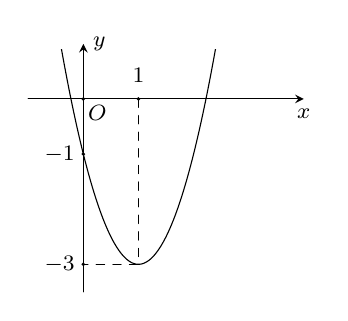
\begin{tikzpicture}[scale=1,>=stealth, font=\footnotesize, line join=round, line cap=round,xscale=.7,yscale=.7]
	\def\a{2} \def\b{-4} \def\c{-1} % Hệ số
	\def\xmin{-1} \def\xmax{4}
	\def\ymin{-3.5} \def\ymax{1}	
	%\draw[color=gray!50,dashed] (\xmin,\ymin) grid (\xmax,\ymax);	
	\draw[->] (\xmin,0)--(\xmax,0) node [below]{$x$};
	\draw[->] (0,\ymin)--(0,\ymax) node [right]{$y$};
	\fill (0,0) circle (1pt) node[shift={(-45:2.5mm)}]{$O$};
	\clip (\xmin+0.1,\ymin+0.1) rectangle (\xmax-0.2,\ymax-0.1);
	\draw[smooth,samples=300,domain=\xmin:\xmax] plot(\x,{\a*(\x)^2+\b*(\x)+\c});
	\foreach \s/\t in {1/90}%Trục Ox
	\fill (\s,0) circle (1pt) node[shift={(\t:3mm)}]{$\s$};
	\foreach \p/\r in {-3/180,-1/180}%Trục Oy
	\fill (0,\p) circle (1pt) node[shift={(\r:3mm)}]{$\p$};
	\draw[dashed] (1,0)|-(0,-3);
\end{tikzpicture}
}
	\loigiai{
	Ta có $2f(x)+3=0 \Leftrightarrow f(x)=-\dfrac{3}{2}$.
	\\
	Từ đồ thị đã cho ta thấy đường thẳng $y=-\dfrac{3}{2}$ cắt đồ thị $(P)$ tại hai điểm phân biệt nên phương trình $2f(x)+3=0$ có hai nghiệm phân biệt.
}
\end{ex}
\begin{ex}%[0D3B1-2]%[Dự án đề kiểm tra HKI NH22-23- Phạm Phương]%[THPT Lương Văn Tụy - Sở Ninh Bình]
	Tập xác định của hàm số $y=\sqrt{x-1}+\dfrac{x}{x-3}$ là
	\choice
	{\True $[1;+\infty) \setminus \{3\}$}
	{$(1;3)$}
	{$(3;+\infty)$}
	{$[1;3)$}
	\loigiai{
	Hàm số $y=\sqrt{x-1}+\dfrac{x}{x-3}$ có nghĩa khi 
	$\heva{& x-1 \geq 0\\& x-3 \neq 0} \Leftrightarrow \heva{& x \geq 1\\& x \neq 3.}$
	\\
	Vậy tập xác định là $\mathscr{D}=[1;+\infty) \setminus \{3\}$.
}
\end{ex}
\begin{ex}%[0H3B1-3]%[Dự án đề kiểm tra HKI NH22-23- Phạm Phương]%[THPT Lương Văn Tụy - Sở Ninh Bình]
	Trong hệ trục tọa độ $Oxy$, cho tam giác $ABC$ có $A(-4;1)$, $B(2;4)$. Tìm tọa độ điểm $C$ sao cho $G(2;-2)$ là trọng tâm của tam giác $ABC$.
	\choice
	{$C(8;11)$}
	{$C(12;11)$}
	{\True $C(8;-11)$}
	{$C(-8;-11)$}
	\loigiai{
	Vì $G$ là trọng tâm của tam giác $ABC$ ta có
	$$\heva{& x_G=\dfrac{x_A+x_B+x_C}{3}\\& y_G=\dfrac{y_A+y_B+y_C}{3}} \Leftrightarrow \heva{& 2=\dfrac{(-4)+2+x_C}{3}\\& -2=\dfrac{1+4+y_C}{3}} \Leftrightarrow \heva{& x_C=8 \\& y_C=-11}\Rightarrow C(8;-11).$$
}
\end{ex}
\begin{ex}%[0H2B4-1]%[Dự án đề kiểm tra HKI NH22-23- Phạm Phương]%[THPT Lương Văn Tụy - Sở Ninh Bình]
	Cho tam giác đều $ABC$ có $I$ là trung điểm của $BC$. Tính góc giữa hai véc-tơ $\overrightarrow{AB}$ và $\overrightarrow{AI}$.
	\choice
	{$\left(\overrightarrow{AB}, \overrightarrow{AI}\right)=45^{\circ}$}
	{$\left(\overrightarrow{AB}, \overrightarrow{AI}\right)=90^{\circ}$}
	{$\left(\overrightarrow{AB}, \overrightarrow{AI}\right)=60^{\circ}$}
	{\True $\left(\overrightarrow{AB}, \overrightarrow{AI}\right)=30^{\circ}$}
	\loigiai{
	\immini{
	Ta có $\left(\vec{AB},\vec{AI}\right)=\widehat{IAB}$.
	\\
	Mà $\triangle ABC$ đều, $AI$ là trung tuyến nên cũng là phân giác suy ra $\widehat{IAB}=30^\circ$. Vậy $\left(\vec{AB},\vec{AI}\right)=30^\circ$.
	}{
	\begin{tikzpicture}[scale=0.8,>=stealth, font=\footnotesize, line join=round, line cap=round]
		\foreach \i/\j/\k in{0/0/B,2/0/C}
		\coordinate (\k) at(\i,\j);
		\path ($(B)!1!60:(C)$) coordinate (A)
		($(B)!0.5!(C)$) coordinate (I);
		\draw (A)--(B)--(C)--cycle
		(A)--(I);
		\foreach \p/\r in {A/90,B/-135,C/-45,I/-90}
		\fill (\p) circle (1pt) node[shift={(\r:2.5mm)}]{$\p$};
		\draw pic[draw=black, mark=|, angle eccentricity=2, angle radius=0.35cm]{angle=B--A--I};
	\end{tikzpicture}
	}
}
\end{ex}
\begin{ex}%[0H2B2-5]%[Dự án đề kiểm tra HKI NH22-23- Phạm Phương]%[THPT Lương Văn Tụy - Sở Ninh Bình]
	Cho tam giác $ABC$ vuông tại $A$ có $AB=3$, $BC=5$. Giá trị của $\left|\overrightarrow{AB}+\overrightarrow{BC}\right|$ là
	\choice
	{$5$}
	{$8$}
	{\True $4$}
	{$3$}
	\loigiai{
		\immini{
	Ta có $\left|\overrightarrow{AB}+\overrightarrow{BC}\right|=\left|\vec{AC}\right|=AC$.
	\\
	$\triangle ABC$ vuông tại $A$ nên $AC=\sqrt{BC^2-AB^2}=\sqrt{5^2-3^2}=4$.
	\\
	Vậy $\left|\overrightarrow{AB}+\overrightarrow{BC}\right|=4$.
}{
\begin{tikzpicture}[scale=0.8,>=stealth, font=\footnotesize, line join=round, line cap=round]
	\foreach \i/\j/\k in{0/0/B,3.5/0/C}
	\coordinate (\k) at(\i,\j);
	\path ($(B)!0.1!53:(C)$) coordinate (Bt)
	($(C)!0.1!-37:(B)$) coordinate (Ct)
	(intersection of B--Bt and C--Ct) coordinate (A)
	;
	\draw (A)--(B)--(C)--cycle;
	\foreach \p/\r in {A/90,C/-45,B/-135}
	\fill (\p) circle (1pt) node[shift={(\r:3mm)}]{$\p$};
	\draw pic[draw=black, angle eccentricity=0.75, angle radius=0.2cm]{right angle=B--A--C};
	\path (A)--(B)node[midway,left]{$3$}	
	(C)--(B)node[midway,below,sloped]{$5$};
\end{tikzpicture}
}
}
\end{ex}
\begin{ex}%[0H3Y1-2]%[Dự án đề kiểm tra HKI NH22-23- Phạm Phương]%[THPT Lương Văn Tụy - Sở Ninh Bình]
	Trong mặt phẳng tọa độ $Oxy$, cho $\vec{a}=(-1;3)$, $\vec{b}=(5;-7)$. Tọa độ véc-tơ $3\vec{a}-2\vec{b}$ là
	\choice
	{$(-6;10)$}
	{$(6;-19)$}
	{\True $(-13;23)$}
	{$(13;-29)$}
	\loigiai{
	Ta có $3\vec{a}-2\vec{b}=\left(3\cdot (-1)-2\cdot 5;3\cdot 3-2\cdot (-7)\right)=\left(-13;23\right)$.
}
\end{ex}
\begin{ex}%[0D3Y2-2]%[Dự án đề kiểm tra HKI NH22-23- Phạm Phương]%[THPT Lương Văn Tụy - Sở Ninh Bình]
	Cho hàm số $y=f(x)$ có bảng biến thiên như hình vẽ sau, chọn khẳng định đúng.
	\begin{center}
		
\begin{tikzpicture}
			\tkzTabInit[nocadre=false,lgt=1.2,espcl=2.5,deltacl=0.6]
			{$x$ /1,$y$ /2}
			{$-\infty$,$-\dfrac{1}{2}$,$+\infty$}
			\tkzTabVar{-/$-\infty$, +/$\dfrac{3}{2}$,-/$-\infty$}
		\end{tikzpicture}
	\end{center}
	\choice
	{Hàm số đồng biến trên khoảng $(2;+\infty)$}
	{Hàm số đồng biến trên khoảng $(-2;+\infty)$}
	{Hàm số nghịch biến trên khoảng $(-\infty;1)$}
	{\True Hàm số nghịch biến trên khoảng $\left(-\dfrac{1}{2};+\infty\right)$}
	\loigiai{
	Từ bảng biến thiên ta suy ra hàm số $y=f(x)$ nghịch biến trên khoảng $\left(-\dfrac{1}{2};+\infty\right)$.
}
\end{ex}
\begin{ex}%[0H2Y4-1]%[Dự án đề kiểm tra HKI NH22-23- Phạm Phương]%[THPT Lương Văn Tụy - Sở Ninh Bình]
	Cho tam giác đều $ABC$ có cạnh bằng $a$. Tính tích vô hướng $\overrightarrow{AB} \cdot \overrightarrow{AC}$.
	\choice
	{$\dfrac{a^2\sqrt{3}}{2}$}
	{$a^2$}
	{\True $\dfrac{a^2}{2}$}
	{$-\dfrac{a^2}{2}$}
	\loigiai{
		\immini{
	Tam giác $ABC$ đều nên $\left(\overrightarrow{AB}, \overrightarrow{AC}\right)= \widehat{BAC}=60^\circ$.
	\\
	$\overrightarrow{AB} \cdot \overrightarrow{AC}=\left|\overrightarrow{AB}\right|\cdot\left|\overrightarrow{AC}\right|\cdot \cos\left(\overrightarrow{AB},\overrightarrow{AC}\right)=a\cdot a \cdot \cos 60^\circ=\dfrac{a^2}{2}$.
	}{
	\begin{tikzpicture}[scale=0.8,>=stealth, font=\footnotesize, line join=round, line cap=round]
		\foreach \i/\j/\k in{0/0/B,2/0/C}
		\coordinate (\k) at(\i,\j);
		\path ($(B)!1!60:(C)$) coordinate (A)
		;
		\draw (A)--(B)--(C)--cycle;
		\foreach \p/\r in {A/90,B/-135,C/-45}
		\fill (\p) circle (1pt) node[shift={(\r:3mm)}]{$\p$};
		\draw pic["$60^\circ$",draw=black, mark=|, angle eccentricity=1.75, angle radius=0.35cm]{angle=B--A--C};
		\path (A)--(B)node[midway,left]{$a$};
	\end{tikzpicture} }
}
\end{ex}
\begin{ex}%[0D2B2-2]%[Dự án đề kiểm tra HKI NH22-23- Phạm Phương]%[THPT Lương Văn Tụy - Sở Ninh Bình]
	\immini{
	Miền không bị gạch (kể cả đường thẳng $d_1$ và $d_2$) là miền nghiệm của hệ bất phương trình nào?
	\choice
	{$\heva{&x+y-1 \leq 0 \\& 2x-y+4 \leq 0}$}
	{$\heva{&x+y-1 \geq 0 \\& 2x-y+4 \leq 0}$}
	{$\heva{&x+y-1 \geq 0 \\& 2x-y+4 \geq 0}$}
	{\True $\heva{&x+y-1 \leq 0 \\& 2x-y+4 \geq 0}$}
}{
	\begin{tikzpicture}[scale=1,>=stealth, font=\footnotesize, line join=round, line cap=round,xscale=.7,yscale=.7]
		\def\xmin{-3} \def\xmax{3.5}
		\def\ymin{-1} \def\ymax{5}
		%\draw[color=gray!50,dashed] (\xmin,\ymin) grid (\xmax,\ymax);	
		\draw[->] (\xmin,0)--(\xmax,0) node [below]{$x$};
		\draw[->] (0,\ymin)--(0,\ymax) node [left]{$y$};
		\fill (0,0) circle (1pt) node[shift={(-135:3mm)}]{$O$};
		\clip (\xmin+0.1,\ymin+0.1) rectangle (\xmax-0.1,\ymax-0.1);
		\draw[smooth,samples=300,domain=\xmin:\xmax] plot(\x,{-(\x)+1});
		\fill[pattern=north east lines,pattern color=gray,opacity=1]plot[domain=\xmin:\xmax](\x,{-(\x)+1})--plot[domain=\xmax:\xmin](\x,{\ymax})--cycle;
		\draw[smooth,samples=300,domain=\xmin:\xmax] plot(\x,{2*(\x)+4});
		\fill[pattern=north east lines,pattern color=gray,opacity=1]plot[domain=\xmin:\xmax](\x,{2*(\x)+4})--plot[domain=\xmax:\xmin](\x,{\ymax})--cycle;
		\fill (1,0) circle (1pt) node[shift={(-135:3mm)}]{$1$};
		\fill (0,1) circle (1pt) node[shift={(-170:3mm)}]{$1$};
		\fill (-2,0) circle (1pt) node[shift={(-70:3mm)}]{$-2$};
		\fill (0,4) circle (1pt) node[shift={(170:3mm)}]{$4$};
		\node at (0.3,4.6)[right]{$d_1$};
		\node at (-3,4)[right]{$d_2$};
	\end{tikzpicture}
	}
	\loigiai{
	Từ hình vẽ ta thấy điểm $O(0;0)$ thuộc miền nghiệm của cả hai bất phương trình nên chỉ có hệ bất phương trình $\heva{&x+y-1 \leq 0 \\& 2x-y+4 \geq 0}$ thoả mãn.
}
\end{ex}
\begin{ex}%[0H2Y2-1]%[Dự án đề kiểm tra HKI NH22-23- Phạm Phương]%[THPT Lương Văn Tụy - Sở Ninh Bình]
	Tính tổng $\overrightarrow{MN}+\overrightarrow{PQ}+\overrightarrow{RN}+\overrightarrow{NP}+\overrightarrow{QR}$.
	\choice
	{$\overrightarrow{PR}$}
	{$\overrightarrow{MR}$}
	{$\overrightarrow{MP}$}
	{\True $\overrightarrow{MN}$}
	\loigiai{
	Ta có $\overrightarrow{MN}+\overrightarrow{PQ}+\overrightarrow{RN}+\overrightarrow{NP}+\overrightarrow{QR}=\overrightarrow{MN}+\overrightarrow{NP}+\overrightarrow{PQ}+\overrightarrow{QR}+\overrightarrow{RN}=\overrightarrow{MN}$.
}
\end{ex}
\begin{ex}%[0D3Y1-3]%[Dự án đề kiểm tra HKI NH22-23- Phạm Phương]%[THPT Lương Văn Tụy - Sở Ninh Bình]
	Cho hàm số $f(x)=\heva{&x^2+3x+1 &\text{khi }x \leq 1 \\& -x+2 &\text{khi } x>1}$. Tính $f(-2)$.
	\choice
	{$0$}
	{$-7$}
	{$4$}
	{\True $-1$}
	\loigiai{
	Vì $-2<1$ nên khi $x=-2$ thì $f(x)=x^2+3x+1$ nên
	$$f(-2)=(-2)^2+3\cdot (-2)+1=-1.$$
}
\end{ex}
\begin{ex}%[0D3B2-1]%[Dự án đề kiểm tra HKI NH22-23- Phạm Phương]%[THPT Lương Văn Tụy - Sở Ninh Bình]
	Cho $(P)\colon y=x^2+bx+c$. Tìm $b$, $c$ biết $(P)$ đi qua $M(-1;8)$ và $(P)$ có trục đối xứng là đường thẳng $x=2$.
	\choice
	{$b=-4$, $c=-3$}
	{$b=4$, $c=-3$}
	{\True $b=-4$, $c=3$}
	{$b=4$, $c=3$}
	\loigiai{
	Vì $(P)$ đi qua $M(-1;8)$ và $(P)$ có trục đối xứng là đường thẳng $x=2$ nên ta có hệ phương trình
	$$\heva{& (-1)^2+b\cdot (-1)+c=8\\& -\dfrac{b}{2\cdot 1}=2} \Leftrightarrow \heva{& -b+c=7\\& b=-4} \Leftrightarrow \heva{& b=-4\\& c=3.}$$
}
\end{ex}
\begin{ex}%[0D3B1-2]%[Dự án đề kiểm tra HKI NH22-23- Phạm Phương]%[THPT Lương Văn Tụy - Sở Ninh Bình]
	Tìm các giá trị thực của tham số $m$ để hàm số $y=\dfrac{x+m+2}{x-m}$ xác định trên $(-1;2)$.
	\choice
	{$\heva{& m \leq-1 \\& m \geq 2}$}
	{$\hoac{& m<-1 \\& m>2}$}
	{\True $\hoac{& m \leq-1 \\& m \geq 2}$}
	{$-1<m<2$}
	\loigiai{
	Hàm số $y=\dfrac{x+m+2}{x-m}$ có nghĩa khi $x-m\neq 0 \Leftrightarrow x\neq m$.
	\\
	Do đó để hàm số đã cho xác định trên $(-1;2)$ thì $m \notin (-1;2) \Rightarrow \hoac{& m\leq-1\\& m\geq 2.}$
}
\end{ex}
\begin{ex}%[0D3K2-5]%[Dự án đề kiểm tra HKI NH22-23- Phạm Phương]%[THPT Lương Văn Tụy - Sở Ninh Bình]
	\immini{
	Một chiếc cổng hình parabol có chiều rộng $AB=8$ m và chiều cao $4$ m bao gồm một cửa chính hình chữ nhật ở chính giữa và hai cánh cửa phụ hai bên (như hình vẽ). Hãy tính chiều cao của cửa chính hình chữ nhật đó biết rằng bề ngang cửa $CD=4$ m.
	}{
	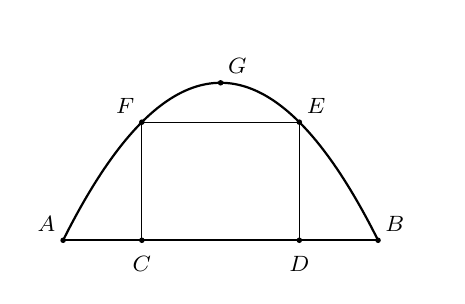
\begin{tikzpicture}[scale=1,>=stealth, font=\footnotesize, line join=round, line cap=round,xscale=0.5,yscale=0.5]
		\def\a{-0.25} \def\b{2} \def\c{0} % Hệ số
		\def\xmin{-1} \def\xmax{10}
		\def\ymin{-1} \def\ymax{5.5}
		%\draw[color=gray!50,dashed] (\xmin,\ymin) grid (\xmax,\ymax);
		\foreach \i/\j/\k in{0/0/A,8/0/B,2/0/C,6/0/D,4/4/G,2/3/F,6/3/E}
		\coordinate (\k) at(\i,\j);
		%\draw[->] (\xmin,0)--(\xmax,0) node [below]{$x$};
		%\draw[->] (0,\ymin)--(0,\ymax) node [left]{$y$};
		%\node at (0,0) [below left]{$O$};
		\clip (\xmin+0.1,\ymin+0.1) rectangle (\xmax-0.5,\ymax-0.1);
		\draw[smooth,samples=300,domain=0:8,thick] plot(\x,{\a*(\x)^2+\b*(\x)+\c});
		\draw (C)--(F)--(E)--(D);
		\draw[thick] (A)--(B);
		\foreach \p/\r in {A/135,B/45,C/-90,D/-90,E/45,F/135,G/45}
		\fill (\p) circle (2pt) node[shift={(\r:3mm)}]{$\p$};
	\end{tikzpicture}
	}
	\choice
	{\True $3$ m}
	{$2{,}5$ m}
	{$2$ m}
	{$3{,}5$ m}
	\loigiai{
	\immini{
	Chọn hệ trục toạ độ $Oxy$ sao cho $O\equiv A$, $B(8;0)$ (như hình bên). Khi đó ta có $C(2;0)$, $D(6;0)$ và $G(4;4)$.
	\\
	Gọi cổng parabol có phương trình dạng $y=ax^2+bx+c$ ta có
	$$\heva{& a\cdot 0^2+b\cdot 0+c=0\\& a\cdot 8^2+b\cdot 8+c=0 \\& a\cdot 4^2+b\cdot 4+c=4} \Leftrightarrow \heva{&c=0 \\& 64a+8b=0 \\& 16a+4b=4} \Leftrightarrow \heva{& a=-\dfrac{1}{4} \\& b=2 \\& c=0.}$$
	}{
	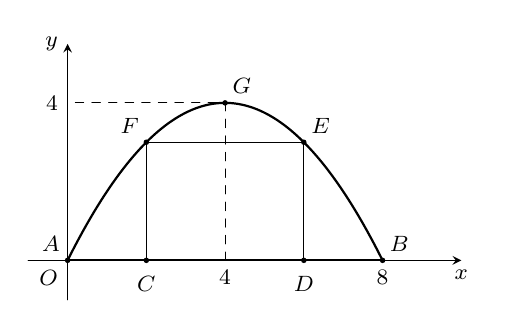
\begin{tikzpicture}[scale=1,>=stealth, font=\footnotesize, line join=round, line cap=round,xscale=0.5,yscale=0.5]
		\def\a{-0.25} \def\b{2} \def\c{0} % Hệ số
		\def\xmin{-1} \def\xmax{10}
		\def\ymin{-1} \def\ymax{5.5}
		%\draw[color=gray!50,dashed] (\xmin,\ymin) grid (\xmax,\ymax);
		\foreach \i/\j/\k in{0/0/A,8/0/B,2/0/C,6/0/D,4/4/G,2/3/F,6/3/E}
		\coordinate (\k) at(\i,\j);
		\draw[->] (\xmin,0)--(\xmax,0) node [below]{$x$};
		\draw[->] (0,\ymin)--(0,\ymax) node [left]{$y$};
		\node at (0,0) [below left]{$O$};
		\clip (\xmin+0.1,\ymin+0.1) rectangle (\xmax-0.5,\ymax-0.1);
		\draw[smooth,samples=300,domain=0:8,thick] plot(\x,{\a*(\x)^2+\b*(\x)+\c});
		\draw (C)--(F)--(E)--(D);
		\draw[thick] (A)--(B);
		\foreach \p/\r in {A/135,B/45,C/-90,D/-90,E/45,F/135,G/45}
		\fill (\p) circle (2pt) node[shift={(\r:3mm)}]{$\p$};
		\node at (B)[below]{$8$};
		\draw[dashed] (4,0)node[below]{$4$}|-(0,4)node[left]{$4$};
	\end{tikzpicture}
	}
	\noindent
	Chiều cao cánh cửa  chính là $y_F=y(2)=-\dfrac{1}{4}\cdot 2^2+2\cdot 2=3$ m.
}
\end{ex}
\begin{ex}%[0H3K2-6]%[Dự án đề kiểm tra HKI NH22-23- Phạm Phương]%[THPT Lương Văn Tụy - Sở Ninh Bình]
	Cho đường tròn tâm $O$ bán kính bằng 5 và hai điểm $A$, $B$ cố định trên đường tròn sao cho $AB=6$. Gọi $M$ là điểm di động trên đường tròn trên, đặt $P=MA^2+2MB^2$. Giả sử $m$, $n$ lần lượt là giá trị lớn nhất và giá trị nhỏ nhất của $P$. Tính giá trị biểu thức $T=m+n$.
	\choice
	{\True $300$}
	{$250$}
	{$320$}
	{$174$}
	\loigiai{
	\immini{
	Gọi $I$ là trung điểm của $AB$ ta có 
	$$OI=\sqrt{OA^2-IA^2}=\sqrt{5^2-3^2}=4.$$
	Đặt hệ trục $Oxy$ như hình vẽ, theo giả thiết đề bài ta có
	$O(0;0)$, $I(0;-4)$, $A(-3;-4)$, $B(3;-4)$.\\
	Đường tròn $(C)$ tâm $O$, bán kính $R=5$ có phương trình dạng $x^2+y^2=25$. Gọi $M(x;y)$ thuộc $(C)$.
	}{
	\begin{tikzpicture}[scale=1,>=stealth, font=\footnotesize,line join=round, line cap=round]
		\def\r{2};
		\path (0,0) coordinate (O)
		(-150:\r) coordinate (A)
		(-30:\r) coordinate (B)
		(120:\r) coordinate (M)
		($(A)!.5!(B)$) coordinate (I)
		;
		\draw[->] (-3,0)--(3,0)node[below]{$x$};
		\draw[->] (0,-2.5)--(0,2.5)node[right]{$y$};		
		\draw (O) circle (\r cm);
		\draw (M)--(A)--(B)--cycle
		(O)--(I)(A)--(O)--(B)
		;
		\draw [dashed] (A)--($(O)!(A)!(1,0)$)node[shift={(90:3mm)}]{$-3$};
		\draw [dashed] (B)--($(O)!(B)!(1,0)$)node[shift={(90:3mm)}]{$3$};
		\foreach \p/\r in {A/180,B/-45,I/-45,M/135,O/135}
		\fill (\p) circle (1pt) node[shift={(\r:3mm)}]{$\p$};
		\node at (I)[shift={(-145:3mm)}]{$-4$};
	\end{tikzpicture}
	}
	\noindent
	Ta có
	\allowdisplaybreaks{
		\begin{eqnarray*}
			P&= &MA^2+2MB^2=\vec{MA}^2+2\vec{MA}^2 \\
			&= &\left(\vec{MO}+\vec{OB}\right)^2+2\left(\vec{MO}+\vec{OB}\right)^2  \\
			&= & \vec{MO}^2+2\vec{MO}\cdot\vec{OA}+\vec{OA}^2+2\vec{MO}^2+4\vec{MO}\cdot\vec{OB}+2\vec{OB}^2 \\
			&= & 6R^2+\vec{MO}\left(2\vec{OA}+4\vec{OB}\right) =150+\vec{MO}\left(2\vec{OA}+4\vec{OB}\right).
	\end{eqnarray*} }
	Lại có
	$$\heva{& \vec{MO}=(-x;-y)\\& 2\vec{OA}+4\vec{OB}=(6;-24)} \Rightarrow \vec{MO}\left(2\vec{OA}+4\vec{OB}\right)=-6x+24y.$$
	Suy ra $P=150-6x+24y \Leftrightarrow 6x-24y-150+P=0 \quad (\Delta)$.\\
	Vì $(\Delta)$ chứa $M$ nên $(\Delta)$ cắt đường tròn $(C)$ tại ít nhất một điểm nên $\Rightarrow \mathrm{d}\left(O,\Delta\right) \leq R$. Do đó
	$$ \dfrac{\left|-150+P\right|}{\sqrt{6^2+(-24)^2}}\leq 5
	\Leftrightarrow  \left|-150+P\right| \leq 30\sqrt{17} 
	\Leftrightarrow 150-30\sqrt{17}\leq P \leq 150+30\sqrt{17}.
	$$
	Vậy giá trị lớn nhất và giá trị nhỏ nhất của $P$ lần lượt là $m=150+30\sqrt{17}$, $n=150-30\sqrt{17}$ suy ra $T=m+n=300$.
}
\end{ex}
\begin{ex}%[0H3K2-6]%[Dự án đề kiểm tra HKI NH22-23- Phạm Phương]%[THPT Lương Văn Tụy - Sở Ninh Bình]
	Trong mặt phẳng tọa độ $Oxy$, cho ba điểm $A(1;0)$, $B(0;5)$, $C(-3;-5)$. Tìm tọa độ điểm $M$ thuộc trục $Oy$ sao cho $|3\overrightarrow{MA}-2 \overrightarrow{MB}+4\overrightarrow{MC}|$ đạt giá trị nhỏ nhất.
	\choice
	{$M(0;-5)$}
	{$M(0;5)$}
	{\True $M(0;-6)$}
	{$M(0;6)$}
	\loigiai{
	$M\in Oy \Rightarrow M(0;m)$. Suy ra $\vec{MA}=(1;-m)$, $\vec{MB}=(0;5-m)$, $\vec{MC}=(-3;-5-m)$.
	\allowdisplaybreaks{
		\begin{eqnarray*}
			\left|3\overrightarrow{MA}-2 \overrightarrow{MB}+4\overrightarrow{MC}\right|&= & \sqrt{\left[3\cdot 1-2\cdot 0+4\cdot (-3)\right]^2+\left[3\cdot(-m)-2\cdot(5-m)+4\cdot (-5-m) \right]^2}\\
			&= & \sqrt{81+(-5m-30)^2}.
	\end{eqnarray*} }
	Biểu thức $|3\overrightarrow{MA}-2 \overrightarrow{MB}+4\overrightarrow{MC}|$ đạt giá trị nhỏ nhất khi $-5m-30=0 \Leftrightarrow m=-6$.\\
	Vậy $M(0;-6)$
}
\end{ex}
\begin{ex}%[0D2K2-2]%[Dự án đề kiểm tra HKI NH22-23- Phạm Phương]%[THPT Lương Văn Tụy - Sở Ninh Bình]
	Cho $x$, $y$ thỏa $\heva{&x-1 \leq 0 \\& y+1 \geq 0 \\& x-y+3 \geq 0}$. Khi đó giá trị lớn nhất của biểu thức $M=2x+y$ bằng bao nhiêu?
	\choice
	{$7$}
	{\True $6$}
	{$9$}
	{$8$}
	\loigiai{
	\immini{
	Miền nghiệm của bất phương trình là miền trong tam giác $ABC$ như hình bên. Khi đó giá trị lớn nhất của biểu thức $M=F(x;y)=2x+y$ đạt được tại các đỉnh của tam giác $ABC$. Ta có
	\begin{itemize}
		\item $F(-4;-1)=2(-4)+(-1)=-9$.
		\item $F(1;-1)=2\cdot 1+(-1)=1$.
		\item $F(1;4)=2\cdot 1+4=6$.
	\end{itemize}
	Vậy giá trị lớn nhất của biểu thức $M=2x+y$ bằng $6$.
	}{
	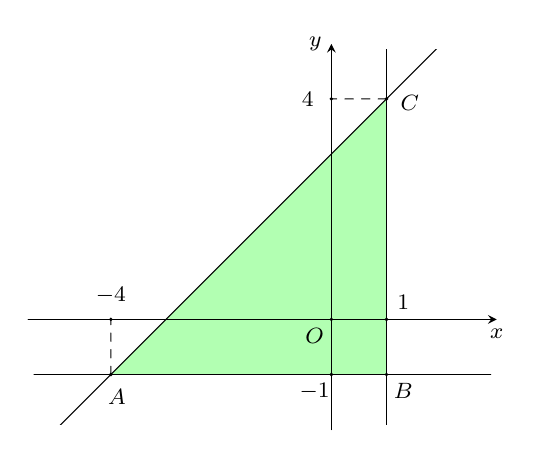
\begin{tikzpicture}[scale=1,>=stealth, font=\footnotesize, line join=round, line cap=round,xscale=.7,yscale=.7]
		\def\xmin{-5.5} \def\xmax{3}
		\def\ymin{-2} \def\ymax{5}
		\foreach \i/\j/\k in{-4/-1/A,1/-1/B,1/4/C}
		\coordinate (\k) at(\i,\j);		
		\fill[green!30] (A)--(B)--(C)--cycle;
		\draw[->] (\xmin,0)--(\xmax,0) node [below]{$x$};
		\draw[->] (0,\ymin)--(0,\ymax) node [left]{$y$};
		\fill (0,0) circle (1pt) node[shift={(-135:3mm)}]{$O$};
		\clip (\xmin+0.1,\ymin+0.1) rectangle (\xmax-0.1,\ymax-0.1);		
		\draw (1,\ymin)--(1,\ymax);
		\draw (\xmin,-1)--(\xmax,-1);
		\draw[smooth,samples=300,domain=\xmin:\xmax] plot(\x,{(\x)+3});
		\draw[dashed] (C)--(0,4)
		(A)--(-4,0)
		;
		\foreach \s/\t in {-4/90,1/45}
		\fill (\s,0) circle (1pt) node[shift={(\t:3mm)}]{$\s$};
		\foreach \p/\r in {-1/-135,4/180}
		\fill (0,\p) circle (1pt) node[shift={(\r:3mm)}]{$\p$};
		\foreach \p/\r in {A/-75,B/-45,C/-10}
		\fill (\p) circle (1pt) node[shift={(\r:3mm)}]{$\p$};
	\end{tikzpicture}
	}
}
\end{ex}
\begin{ex}%[0D3B2-3]%[Dự án đề kiểm tra HKI NH22-23- Phạm Phương]%[THPT Lương Văn Tụy - Sở Ninh Bình]
	\immini{
	Cho hàm số bậc hai $y=ax^2+bx+c$ có đồ thị là đường parabol như hình vẽ. Khẳng định nào sau đây là đúng?
	\choice
	{$a>0$, $b<0$, $c>0$}
	{$a<0$, $b>0$, $c>0$}
	{\True $a<0$, $b<0$, $c<0$}
	{$a<0$, $b>0$, $c<0$}
}{
	\begin{tikzpicture}[scale=1,>=stealth, font=\footnotesize, line join=round, line cap=round,xscale=.7,yscale=.7]
		\def\a{-4/9} \def\b{-4/3} \def\c{-1.5} % Hệ số
		\def\xmin{-4} \def\xmax{1}
		\def\ymin{-2.5} \def\ymax{1}	
		%\draw[color=gray!50,dashed] (\xmin,\ymin) grid (\xmax,\ymax);	
		\draw[->] (\xmin,0)--(\xmax,0) node [below]{$x$};
		\draw[->] (0,\ymin)--(0,\ymax) node [right]{$y$};
		\fill (0,0) circle (1pt) node[shift={(-45:2.5mm)}]{$O$};
		\clip (\xmin+0.1,\ymin+0.1) rectangle (\xmax-0.2,\ymax-0.1);
		\draw[smooth,samples=300,domain=\xmin:\xmax] plot(\x,{\a*(\x)^2+\b*(\x)+\c});
	\end{tikzpicture}
	}
	\loigiai{
		Từ hình vẽ đã cho ta có
\begin{itemize}
	\item Parabol có bề lõm hướng xuống nên $a<0$.
	\item Parabol cắt trục tung tại điểm có tung độ âm nên $c<0$.
	\item Đỉnh parabol có hoành độ âm nên $-\dfrac{b}{2a}<0$ hay $a$, $b$ cùng dấu suy ra $b<0$.
\end{itemize}
Vậy $a<0$, $b<0$, $c<0$.
}
\end{ex}

\Closesolutionfile{ans}
%\begin{center}
%	\textbf{ĐÁP ÁN}
%	\inputansbox{10}{ans/ans}	
%\end{center}


\begin{center}
	\textbf{PHẦN 2 - TỰ LUẬN}
\end{center}

\begin{bt}%[0D3Y1-2]%[HKI NH22-23, TheHung Nguyen]%[THPT LƯƠNG VĂN TỤY, NINH BÌNH]
	Tìm tập xác định $\mathrm{D}$ của hàm số $y=\dfrac{x+1}{2x-2}$.
	\loigiai{Điều kiện $2x-2\ne 0\Leftrightarrow x\ne 1$.\\
		Tập xác định $\mathscr{D}=\mathbb{R}\backslash\{1\}$ 
	}
\end{bt}



\begin{bt}%[0D3K2-4]%[0D3B2-4]%[HKI NH22-23, TheHung Nguyen]%[THPT LƯƠNG VĂN TỤY, NINH BÌNH]
	\text{}
	\begin{enumerate}
		\item Vẽ đồ thị hàm số $y=x^2-2x-3$.			
		\item Tìm tất cả giá trị thực của tham số $m$ sao cho parabol $(P)\colon y=x^2-4 x+m$ cắt $O x$ tại hai điểm phân biệt $A, B$ thỏa mãn $OA=3OB$.
	\end{enumerate}
\loigiai{
	\begin{enumerate}
	\item Vẽ đồ thị hàm số $y=x^2-2 x-3$.
		\begin{enumerate}[$ \star $]
			\item Tập xác định $\mathscr{D}=\mathbb{R}.$
			\item Trục đối xứng $x=1$.
			\item Tọa độ đỉnh $I(1;-4)$.		
			\item Đồ thị
			\begin{center}
				\begin{tikzpicture}[scale=.75, font=\footnotesize, line join=round, line cap=round, >=stealth]
					\def\xmin{-2}\def\xmax{4}\def\ymin{-4.5}\def\ymax{1}
					\draw[->] (\xmin-0.2,0)--(\xmax+0.2,0) node[below] {\footnotesize $x$};
					\draw[->] (0,\ymin-0.2)--(0,\ymax+0.2) node[right] {\footnotesize $y$};
					\draw (0,0) node [below left] {\footnotesize $O$};
					\foreach \x in {2,3,4}\draw (\x,0.1)--(\x,-0.1) node [below] {\footnotesize $\x$};
					\foreach \x in {1}\draw (\x,0.1)--(\x,-0.1) node [above] {\footnotesize $\x$};
					\foreach \x in {-1}\draw (\x,0.1)--(\x,-0.1) node [ below left] {\footnotesize $\x$};
					\foreach \y in {-4,-3,-1,1}\draw (0.1,\y)--(-0.1,\y) node [left] {\footnotesize $\y$};
					\clip (\xmin,\ymin) rectangle (\xmax,\ymax);
					\draw[smooth,samples=200,domain=\xmin:\xmax] plot (\x,{1*((\x)^2)+-2*\x+-3});
					\draw[dashed] (1.0,0)--(1.0,-4.0)--(0,-4.0);\fill (1.0,-4.0) circle (1pt);
				\end{tikzpicture}
			\end{center}
		\end{enumerate}
	\item Phương trình hoành độ giao điểm của $(P)$ và $Ox$ là $$x^2-4x+m=0\qquad(1).$$
	Để $(P)$ cắt $O x$ tại hai điểm phân biệt thì $(1)$ có hai nghiệm phân biệt $x_1$, $x_2$
$$\heva{&{\Delta'>0}\\ &{a\neq 0}}\Leftrightarrow\heva{&4-m>0\\ &1\neq 0}\Leftrightarrow m<4 .$$
	Giả sử $A\left(x_1 ; 0\right)$, $B\left(x_2 ; 0\right)$ và $x_1+x_2=4$, $x_1 x_2=m$.\\
	Ta có
	$O A=3O B\Leftrightarrow\left|x_1\right|=3\left|x_2\right|\Leftrightarrow\hoac{&x_1=3x_2\\ &x_1=-3x_2.}$\\
	\textbf{Trường hợp 1:} $x_1=3x_2\Rightarrow\heva{&x_1=3\\ &x_2=1}\Rightarrow m=3\text{~(thỏa mãn)}$.\\
	\textbf{Trường hợp 2:} $x_1=-3x_2\Rightarrow\heva{&x_1=6\\ &x_2=-2}\Rightarrow m=-12\text{~(thỏa mãn)}$.\\	
	Vậy $m\in \{-12;3\}$ thỏa đề bài.	
\end{enumerate}
}
\end{bt}

\begin{bt}%[0H2B4-1]%[HKI NH22-23, TheHung Nguyen]%[THPT LƯƠNG VĂN TỤY, NINH BÌNH]
	\text{}
	\begin{enumerate}
		\item Cho tam giác $ABC$ vuông cân tại $A$ có cạnh bằng $AB=AC=2$. Tính tích vô hướng $\overrightarrow{B A} \cdot \overrightarrow{B C}$.
		\item Trong mặt phẳng tọa độ $O x y$, cho tam giác $A B C$ có $A(1 ; 2), B(2 ;-1), C(2 ; 4)$. Tính số đo góc $A$ của tam giác đã cho.
	\end{enumerate}
\loigiai{
	\begin{enumerate}
	\item Ta có $BC^2=AB^2+AC^2\Rightarrow BC=\sqrt{2^2+2^2}=2\sqrt{2}$.
	\immini{Ta có $\overrightarrow{B A} \cdot \overrightarrow{B C}= BA\cdot BC\cdot \cos B=2\cdot 2\sqrt{2}\cdot \cos 45^\circ =4$.
	}{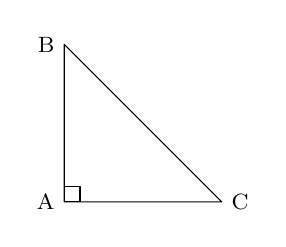
\begin{tikzpicture}[scale=1, font=\footnotesize, line join=round, line cap=round, >=stealth]
			\draw (0,0) node[left] {A} -- (2,0) node[right] {C} -- (0,2) node[left] {B} -- cycle;
			\draw (0,0) rectangle (0.2,0.2);
	\end{tikzpicture}}
	\item Ta có\\
	 $\overrightarrow{AB}= (1;-3)\Rightarrow AB=\sqrt{1^2+(-3)^2}=\sqrt{10}$.\\
	$\overrightarrow{AC}= (1;2)\Rightarrow AC=\sqrt{1^2+2^2}=\sqrt{5}$.\\
	$\overrightarrow{BC}= (0;5)\Rightarrow BC=\sqrt{0^2+5^2}=5$.\\
	Áp dụng định lý hàm số cos trong tam giác $ABC$, ta có\\
	$$\cos A=\dfrac{AB^2+AC^2-BC^2}{2AB\cdot AC}=\dfrac{10+5-25}{100}=-\dfrac{\sqrt{2}}{2}\Rightarrow A=135^\circ.$$	
	\end{enumerate}
}
\end{bt}

